\section{Time de medição (Time GQM)}

	O time que realizará as medições, bem como executar o presente plano, é composto pelos seguintes integrantes,
	sendo os dois primeiros integrantes componentes da equipe de gerência do projeto alvo:

	\begin{itemize}
	 \item Emilie Morais;
	 \item Ítalo Paiva;
	 \item Leonardo Cambraia;
	 \item Lucas Costa;
	 \item Omar Faria.
	\end{itemize}

	O comprometimento com o processo de medição é facilmente estabelecido, uma vez que dois integrantes do time de GQM
	fazem parte da gerência do projeto em questão.

    \section{Escopo da medição e caracterização da organização}

      A organização e o projeto que serão tratados neste plano estão descritos nas seções
      \ref{organizacao} e \ref{diagnostico}, respectivamente.

      \subsection{Área de melhoria}

	A organização deseja melhorar as taxas de entregas dos incrementos de \textit{software} nas \textit{sprints}, evitando os
	atrasos, diminuindo assim os custos e riscos para o projeto.


    \section{Programa de medição}

      Para a elaboração do seguinte programa de medição, foi adotado o modelo proposto pelo método GQM (apresentado na seção \ref{gqm}),
      com algumas considerações da Norma ISO/IEC 15939:2007 (apresentada na seção \ref{15939}).

      \subsection{Objetivos de medição}

	Para o presente trabalho foi definido o objetivo de medição descrito na Tabela \ref{objetivo_medicao}.

	\begin{table}[!htb]
	  \centering
	  \caption{Objetivo de medição}
	  \label{objetivo_medicao}
	  \begin{tabular}{|l|l|}
	  \hline
	  \textbf{Analisar}                                                           & as entregas de incremento de software por Sprint \\ \hline
	  \textbf{\begin{tabular}[c]{@{}l@{}}Com o \\ propósito de\end{tabular}}      & melhorar                                         \\ \hline
	  \textbf{Com respeito a}                                                     & atrasos                                          \\ \hline
	  \textbf{\begin{tabular}[c]{@{}l@{}}Sob o ponto \\ de vista de\end{tabular}} & gerentes de projeto                           \\ \hline
	  \textbf{No contexto de}                                                     & projeto proposto de GPP/MDS \\ \hline
	  \end{tabular}
	\end{table}

      \subsection{Questões}

	Refinando o objetivo de medição definido, obteve-se as seguintes questões:

	\begin{itemize}

	 \item \textbf{Q1}. \textit{Qual a influência da procrastinação no atraso das entregas?}
		\subitem A procrastinação gera postergação do trabalho que resulta em sobrecarga ao final da sprint, podendo provocar atraso da entrega das atividades.

	 \item \textbf{Q2}. \textit{Qual a influência dos erros das estimativas no atraso das entregas?}
		\subitem Os erros das estimativas provocam prejuízo no entendimento do valor de cada história, prejudicando a divisão das histórias, o valor do trabalho, além de gerar falso entendimento sobre o estado atual do projeto, aumentando a chance de provocar atraso na entrega.

	 \item \textbf{Q3}. \textit{Qual a influência da dificuldade na linguagem no atraso das entregas?}
		\subitem A falta de domínio da linguagem diminui a noção de trabalho que pode ser realizado em determinado tempo, por não se compreender completamente o contexto em que se está trabalhando, aumentando a chance de encontrar novos obstáculos, tendo que despender mais tempo do que o planejado para resolve-los, podendo provocar atrasos na entrega.

	 \item \textbf{Q4}. \textit{Qual a influência da dificuldade de comunicação no atraso das entregas?}
		\subitem Através da comunicação, o time pode se planejar corretamente e se adequar aos problemas reais da sprint. A dificuldade de comunicação proporciona falta de conhecimento sobre o estado estado atual da sprint, caso a percepção de trabalho a realizar seja maior que a esperada pelo time, aumenta a chance de atraso na entrega.

	\end{itemize}


      \subsection{Métricas}

	Refinando as questões definidas na subseção anterior, obteve-se as seguintes métricas:

	\begin{itemize}

	 \item \textbf{M1}. \textit{Velocity} diário

	   \subitem \textbf{Descrição}: Esta métrica consiste na quantidade pontos que é realizado por dia pelo time.

	   \subitem \textbf{Unidade}: \textit{Story Points}/dia.

	   \subitem \textbf{Forma de coleta}: Acompanhamento diário da produção por planilha online.

	   \subitem \textbf{Questões respondidas}: Esta métrica ajuda a responder à Questão Q1, pois permite acompanhar o quanto
		    foi produzido por dia, proporcionando a avaliação de quando o time começou a trabalhar. Esta métrica pode ser
		    graficamente acompanhada a partir do gráfico de \textit{burndown}. Esta métrica também é usada para calcular a
		    métrica M2, para realizar a análise proposta.

	 \item \textbf{M2}. Média de pontos realizados por dia

	   \subitem \textbf{Descrição}: Esta métrica é derivada da métrica M1.\textit{Velocity} diário. Consiste na média das velocidades
		    diárias.

	   \subitem \textbf{Unidade}: \textit{Story Points}/dia.

	   \subitem \textbf{Forma de coleta}: Derivada da coleção de métricas M1.

	      \subsubitem \textbf{Fórmula:}

		$$ M2 = (\sum\limits_{i=1}^{n}M1_i)/n $$

	      \subsubitem Onde $n = quantidade\ de\ dias$.

	   \subitem \textbf{Questões respondidas}: Esta métrica ajuda a responder à Questão Q1, pois informa a quantidade média do
		    que a equipe consegue produzir por dia, servindo para realizar análise proposta para o fator de procrastinação.

	 \item \textbf{M3}. Pontos planejados por \textit{sprint}

	   \subitem \textbf{Descrição}: Esta métrica consiste na quantidade de pontos que foram alocados para cada \textit{sprint}.

	   \subitem \textbf{Unidade}: \textit{Story Points}.

	   \subitem \textbf{Forma de coleta}: Realizando o \textit{planning poker} no planejamento de cada \textit{sprint}
		    cujos dados são documentados numa planilha online.

	   \subitem \textbf{Questões respondidas}: Esta métrica ajuda a responder às Questões Q1 e Q2, pois fornece os dados para
		    calcular a média dos pontos planejados por \textit{sprint} (M4) que será utilizada para a análise do impacto
		    da procrastinação e dos erros nas estimativas.

	 \item \textbf{M4}. Média de pontos alocados por \textit{sprint}

	   \subitem \textbf{Descrição}: Esta métrica é derivada da métrica M3.Pontos planejados por \textit{sprint}.
		    Consiste na média dos pontos que são planejados por \textit{sprint}, indicando a quantidade média
		    de pontos que são alocados.

	   \subitem \textbf{Unidade}: \textit{Story Points}.

	   \subitem \textbf{Forma de coleta}: Derivada da coleção de métricas M3.

	      \subsubitem \textbf{Fórmula:}

		$$ M4 = (\sum\limits_{i=1}^{n}M3_i)/n $$

	      \subsubitem Onde $n = quantidade\ de\ sprints$.

	   \subitem \textbf{Questões respondidas}: Esta métrica ajuda a responder às Questões Q1 e Q2, pois permite a análise
		    proposta para os fatores de procrastinação e de erros nas estimativas.

	 \item \textbf{M5}. Pontuação das histórias

	   \subitem \textbf{Descrição}: Esta métrica consiste na pontuação inicial de cada história definida no \textit{backlog} no início
		    da \textit{sprint} (na reunião de planejamento).

	   \subitem \textbf{Unidade}: \textit{Story Points}.

	   \subitem \textbf{Forma de coleta}: Realizando o \textit{planning poker} no planejamento da \textit{sprint}
		    cuja história foi alocada. Os dados são documentados numa planilha online.

	   \subitem \textbf{Questões respondidas}: Esta métrica ajuda a responder à Questão Q2, pois fornece parte do insumo para calcular
		    as métricas M7 e M8.

	 \item \textbf{M6}. Repontuação das histórias

	   \subitem \textbf{Descrição}: Esta métrica consiste na pontuação final de cada história definida no \textit{backlog} no fim
		    da \textit{sprint} (na reunião de retrospectiva).

	   \subitem \textbf{Unidade}: \textit{Story Points}.

	   \subitem \textbf{Forma de coleta}: Realizando a repontuação utilizando o \textit{planning poker} na retrospectiva da \textit{sprint}
		    cuja história foi alocada. Os dados são documentados numa planilha online.

	   \subitem \textbf{Questões respondidas}: Esta métrica ajuda a responder à Questão Q2, pois fornece a outra parte do insumo para calcular
		    as métricas M7 e M8.

	 \item \textbf{M7}. Erro na estimativa por história

	   \subitem \textbf{Descrição}: Esta métrica é derivada das métricas M5.Pontuação das histórias e M6.Repontuação das histórias.
		    Consiste na diferença entre os pontos obtidos com a repontuação e os pontos da pontuação inicial.

	   \subitem \textbf{Unidade}: \textit{Story Points}.

	   \subitem \textbf{Forma de coleta}: Derivada das métricas M5 e M6.

	      \subsubitem \textbf{Fórmula:}

		$$ M7_i = M6_i - M5_i $$

	      \subsubitem Onde $i = número\ da\ história\ referente\ às\ métricas$

	   \subitem \textbf{Questões respondidas}: Esta métrica ajuda a responder à Questão Q2, pois permite parte da análise
		    dos erros nas estimativas.

	 \item \textbf{M8}. Precisão da estimativa

	   \subitem \textbf{Descrição}: Esta métrica é derivada das métricas M5.Pontuação das histórias e M6.Repontuação das histórias.
		    Consiste na razão entre os pontos obtidos com a repontuação e os pontos da pontuação inicial. É uma métrica adicional
		    para acrescentar outro ponto de vista para o erro nas estimativas.

	   \subitem \textbf{Unidade}: Adimensional.

	   \subitem \textbf{Forma de coleta}: Derivada das métricas M5 e M6.

	      \subsubitem \textbf{Fórmula:}

		$$ M8_i = M6_i / M5_i $$

	      \subsubitem Onde $i = número\ da\ história\ referente\ às\ métricas$.

	   \subitem \textbf{Questões respondidas}: Esta métrica está atrelada à Questão Q2, pois permite um outro ponto de vista
		    para análise dos erros nas estimativas.

	 \item \textbf{M9}. Erro médio nas estimativas

	   \subitem \textbf{Descrição}: Esta métrica é derivada da métrica M7.Erro na estimativa por história.
		    Consiste na média dos erros obtidos.

	   \subitem \textbf{Unidade}: \textit{Story Points}.

	   \subitem \textbf{Forma de coleta}: Derivada das métricas M7.

	      \subsubitem \textbf{Fórmula:}

		$$ M9 = (\sum\limits_{i=1}^{n}M7_i)/n $$

	      \subsubitem Onde $n = quantidade\ de\ histórias$.

	   \subitem \textbf{Questões respondidas}: Esta métrica ajuda a responder à Questão Q2, pois permite a análise
		    dos erros nas estimativas, fornecendo um valor médio para os erros.

	 \item \textbf{M10}. \textit{Velocity} da equipe por \textit{sprint}

	   \subitem Explicar a métrica, informando a unidade de medida o método de coleta dessa métrica. Dizer quais questões essa
		    métrica ajuda a responder.

	 \item \textbf{M11}. Percepção do time sobre a linguagem

	   \subitem Explicar a métrica, informando a unidade de medida o método de coleta dessa métrica. Dizer quais questões essa
		    métrica ajuda a responder.

	 \item \textbf{M12}. Percepção do time sobre a comunicação

	   \subitem Explicar a métrica, informando a unidade de medida o método de coleta dessa métrica. Dizer quais questões essa
		    métrica ajuda a responder.

	    \subitem \textbf{Descrição}: Esta métrica representa o grau de percepção do time sobre a comunicação. O conhecimento sobre o estado atual da sprint, os problemas que as duplas estão enfrentando e qual o progresso realizado. O estado atual da comunicação se pode dar em três estados: ruim, boa ou ótima. Para o caso ruim, o time não tem noção do que esta acontecendo dentro de cada par de desenvolvimento, qual o progresso realizado, ou quais problemas estão enfrentando. Para o caso bom, o time se comunica de forma simples sem transparecer o real problema, as duplas tem noção do progresso geral do time através do burndown. No estado ótimo, as duplas se comunicam e compreendem o progresso e problemas de cada uma.

	   \subitem \textbf{Unidade}: Adimensional.

	   \subitem \textbf{Forma de coleta}: Na reuniões diárias e de retrospectivas.

	   \subitem \textbf{Questões respondidas}: Esta métrica está atrelada à Questão Q4, ela tenta expressar em qual estado a comunicação do time se encontra. Para então propor juntamente com o time de desenvolvimento formas de melhorar a comunicação.

	\end{itemize}

      \vfill
      \pagebreak
      \subsection{Modelo GQM proposto}

	A Figura \ref{gqm_proposto} ilustra o modelo do programa de medição proposto, contendo o objetivo de medição, as
	questões associadas e suas respectivas métricas.

	\begin{figure}[!htb]
	  \centering
	  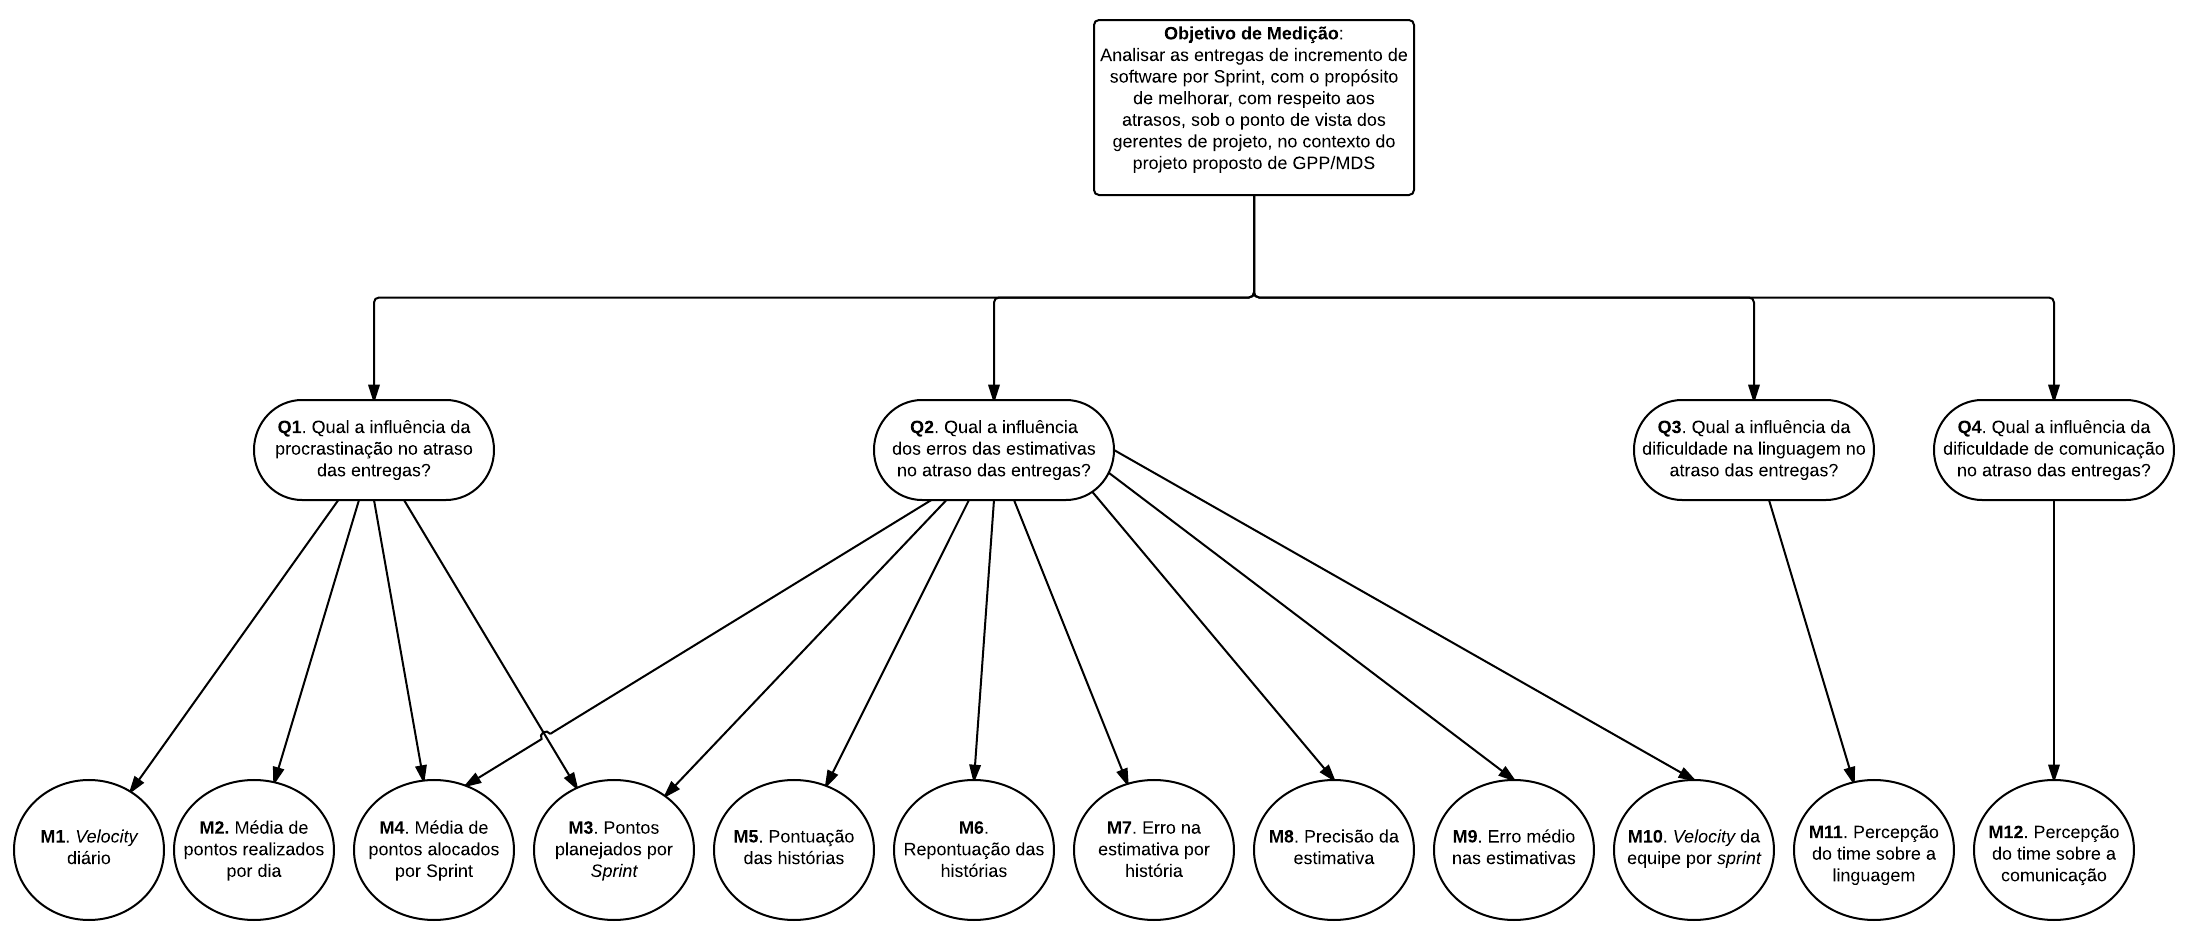
\includegraphics[scale=0.27, angle=90]{figuras/GQM}
	  \caption[Modelo do GQM proposto.]{Modelo do GQM proposto.}
	  \label{gqm_proposto}
	\end{figure}

    \section{Procedimentos}

      Esta seção descreve os procedimentos que devem ser adotados para coleta e análise de dados, e comunicação dos resultados obtidos.

      \subsection{Coleta de dados}

      Para a coleta de dados serão realizadas aplicações de questionário no grupo de GPP e MDS em questão onde cada integrante contribuirá com suas respostas expressando suas percepções acerca do trabalho ao qual está sendo desenvolvido pela equipe.

      Outra maneira que será eficaz na coleta de dados é no planejamento da Sprint. Serão coletadas métricas como os pontos planejados por \textit{sprint} (M3), pontuação das histórias (M5) e repontuação das histórias (M6). Essas métricas coletadas no planejamento da \textit{sprint} são coletadas através do \textit{planning poker} - técnica utilizada para realizar a pontuação de histórias.

      Outro modo que consistirá na coleta de dados será na realização de reuniões diárias. Essas reuniões consistem em encontros rápidos que tem a função de alinhar o andamento da sprint. As métricas coletadas neste tipo de encontro consistem em \textit{velocity} diário (M1).

      Além desses dois, as retrospectivas também são de suma importância para a coleta de dados que visa auxiliar a análise desejada. Nesta reunião serão coletadas métricas como o \textit{velocity} da equipe por \textit{sprint} (M10), a percepção do time sobre a linguagem (M11) e a percepção do time sobre a comunicação (M12).

      As coletas são documentadas em uma planilha online utilizando-se a ferramenta online do _Google_ (_Drive_).

      \subsection{Análise dos dados}

      	Nesta subseção serão descritas as regras para a análise dos dados coletados, de forma a responder às questões definidas.

      	\subsubsection{Questão Q1}

      		\textbf{Métricas envolvidas}: M1, M2, M3 e M4.

      		Esta questão será respondida calculando a métrica M2, a partir dos valores da métrica M1, e a métrica M4, a partir dos valores
      		da métrica M3.

      		Para uma análise geral do projeto, será realizada uma simulação do andamento da \textit{sprint} considerando uma quantidade de
      		pontos definida pela métrica M4.Média de pontos alocados por \textit{sprint}, e utilizando o valor da métrica M2.Média de pontos realizados por dia para a queima dos pontos durante a \textit{sprint}, simulando o começo do trabalho no início da \textit{sprint}.

      		Na simulação citada, caso a quantidade média de pontos alocados na \textit{sprint} tenham sido cumpridos considerando
      		o \textit{velocity} diário médio, temos que a procrastinação do trabalho durante a \textit{sprint} implicou
      		consideravelmente nos atrasos.

      		A simulação também pode ser feita variando o dia de início das atividades.

      		A análise pode ser realizada por \textit{sprint}, utilizando apenas o valor da métrica M3 da \textit{sprint} desejada, ao invés da métrica M4.

      \subsection{Comunicação dos resultados}